\documentclass[12pt]{article}
\usepackage[utf8]{vietnam}
\usepackage{amsmath,amssymb}
\usepackage{tikz}
\usetikzlibrary{calc,angles,intersections,patterns,3d}
% Tạo môi trường vd đánh số tự động cho các Ví dụ
\newtheorem{vd}{\bfseries Ví dụ}
\title{Horner và Bêzout}
\author{Phạm Đăng Long}
\newcounter{sobc}
\newcommand{\hsdathuc}[2]{
	\setcounter{sobc}{0}
	\def\a{{#1}}
	\foreach \i in {#1}{\stepcounter{sobc}\thesobc}
	\def\n{\thesobc}
	\pgfmathsetmacro{\bac}{\n-1}
	\pgfmathsetmacro{\bact}{\n-2}
	\foreach \i in {0,...,\bac}{
		\pgfmathsetmacro{\hsa}{int(\a[\i])}
		\path (\i,0) node {$\hsa$};
	}
	\pgfmathsetmacro{\hsb}{int(\a[0])}
	\path (0,-1) node {$\hsb$};
	\foreach \i [evaluate=\i as \hsb using int(\myglobalfactorial *#2), remember=\hsb as \myglobalfactorial (initially 1)] in {1,...,\bac}{
		\pgfmathsetmacro{\hsb}{int(\hsb +\a[\i])}
		\path (\i,-1) node{$\hsb$};
	}
	\path (-1,-1) node{$#2$};
	\draw (-1.5,-1.5) rectangle (\bac+0.5,0.5) (-1.5,-0.5)--(\bac+0.5,-0.5);
	\foreach \i in {-1,...,\bact}{\draw (\i+0.5,0.5)--(\i+0.5,-1.5);}
}
%=============
\begin{document}
	\maketitle
	Để tính giá trị của đa thức $P(x)=ax^3+bx^2+cx+d$, ta làm theo cách của Horner là $P(x) = ((ax + b)x + c)x + d$. Các đa thức bậc cao hơn nữa cũng làm tương tự. Horner đưa ra lược đồ dễ làm để tính $P(\alpha)$. Và đây là công thức cho bậc ba nói trên:
	%\section{}
	\begin{center}
		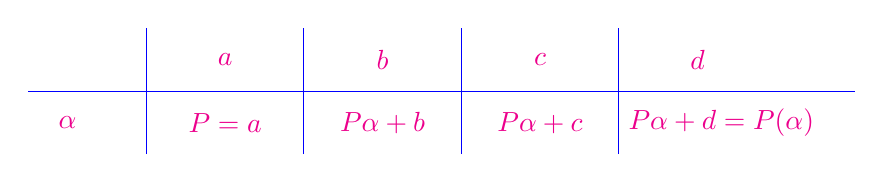
\begin{tikzpicture}[xscale=2,yscale=.8]
			\path[magenta]
			(0,0) node{$\alpha$}
			++(0:1) node{$P=a$} +(90:1) node{$a$}
			++(0:1) node{$P\alpha+b$} +(90:1) node{$b$}
			++(0:1) node{$P\alpha+c$} +(90:1) node{$c$}
			++(0:1) node[right=-1cm]{$P\alpha+d=P(\alpha)$} +(90:1) node{$d$};
			\draw[blue]
			(-.25,.5)--+(0:5.25)
			(.5,-.5)--+(90:2)
			(1.5,-.5)--+(90:2)
			(2.5,-.5)--+(90:2)
			(3.5,-.5)--+(90:2);
		\end{tikzpicture}
	\end{center}
	{\noindent\bfseries Ví dụ 1.} Chia $x^3+x^2-12$ cho $x+2$ (khuyết $x$).
	\begin{center}
		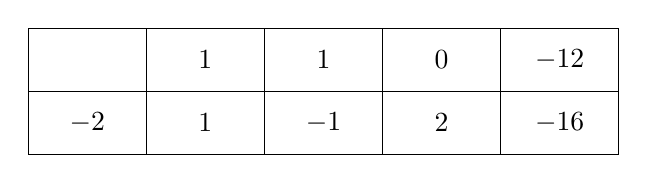
\begin{tikzpicture}[xscale=1.5,yscale=.8]
			\hsdathuc{1,1,0,-12}{-2}
		\end{tikzpicture}
	\end{center}
	\noindent tức là $(x^3+x^2-12):(x+2)$ được $(x^2-x+2)$ dư $-16$.
	{\noindent\bfseries Ví dụ 2.} Chia $x^{3}-x-10$ cho $x-2$ (khuyết $x^{2}$).
	\begin{center}
		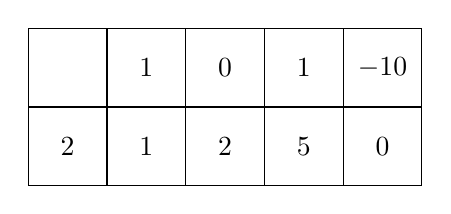
\begin{tikzpicture}
			\hsdathuc{1,0,1,-10}{2};
		\end{tikzpicture}
	\end{center}
	\noindent tức là $(x^{3}-x-10):(x-2)$ đươck $x^{2}+x-10$ (không dư), hay $2$ là một nghiệm của $x^{3}-x-10$.
	{\noindent\bfseries Ví dụ 3.} Ta hoàn toàn có thể chia các đa thức bậc bất kì $P(x)$ cho các nhị thức dạng $x-\alpha$. Chẳng hạn tôi chia đa thức $P(x)=2x^{4}-4x^{2}-2$ cho $x+1$:
	\begin{center}
		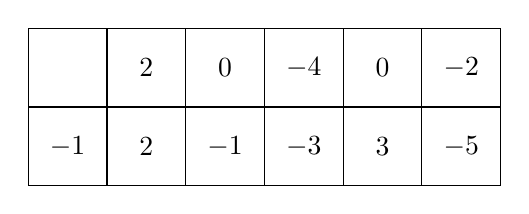
\begin{tikzpicture}
			\hsdathuc{2,0,-4,0,-2}{-1};
		\end{tikzpicture}
	\end{center}
	\noindent Hoặc bậc cao hơn nữa: Chia $P(x)=-3x^{6}+2x^{4}-x^{3}+x^{2}-x+1$ cho $x-2$
	\begin{center}
		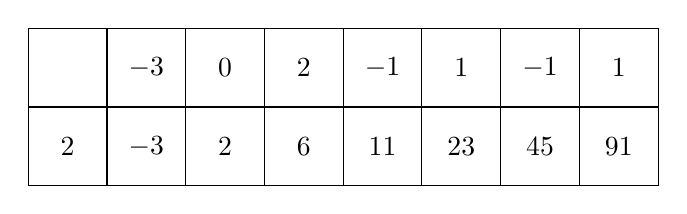
\begin{tikzpicture}
			\hsdathuc{-3,0,2,-1,1,-1,1}{2};
		\end{tikzpicture}
	\end{center}
\end{document}